\section{Caso de estudio: Oficina de Relaciones Internacionales de la Facultad de Filosofía y Letras de la Universidad de Granada}
\subsection{Sobre la oficina}
La labor principal de la oficina es encargarse de la gestión de los programas de intercambio y la movilidad de los estudiantes e incluso de profesores. Como no podía ser de otra manera, proporcionan la información necesaria para los interesados en estos programas, tanto de fuera de la UGR como desde universidades extranjeras. Es más, también revisan convenios existentes con éstas y hacen otros nuevos para ofrecer cada vez más alternativas para poder mejorar nuestra formación.

En su día a día, atienden peticiones y dudas de los estudiantes que participan en alguno de los citados programas; es más, se dedican a asesorar y mostrar todas las alternativas de las que disponen cuando se nos presenta alguna situación complicada, de modo que podamos resolverlo de la forma en que más nos beneficie. Trabajan, en definitiva, con el futuro de los estudiantes, pues la movilidad la desarrollamos con el objetivo de complementar nuestra formación, algo fundamental y abrumador al mismo tiempo cuando se cruzan fronteras y se quiere seguir en el camino de la educación en una universidad que no es la de casa.

La oficina se sitúa junto a la secretaría, en la Facultad de Filosofía y Letras de la Universidad de Granada, en el Campus de Cartuja, y en ella trabajan alrededor de cuatro personas. Es, dadas las cifras que se tienen, una gran cantidad de información las que tan sólo unas pocas personas tienen que manejar con una herramienta que ha sido creada sobre la marcha para facilitar su importante labor; un trabajo que no puede parar ni tolera fallos, pues los estudiantes de movilidad son uno de los pilares fundamentales de la institución.

\subsection{Servicio al estudiantado}
\subsubsection{Estudiantes salientes o \textit{outcoming}}

En relación con los estudiantes salientes, en la oficina se encargan de coordinar a los tutores académicos, que son quienes revisan los acuerdos de estudios que los candidatos proponen para iniciar su movilidad. Una vez éstos les han dado el visto bueno, en la oficina revisan cada uno de los mismos para asegurarse de que todo está en orden. Una vez iniciada la movilidad puede darse el caso en que el/la estudiante desee hacer alguna modificación a su acuerdo, debido a algún cambio imprevisto o a que alguna asignatura no fuera como se esperaba, todo ello en el destino. En ese caso, el proceso sería el mismo: tendrían que volverse a revisar de nuevo los documentos para comprobar que todo está en orden.

También escuchan casos de estudiantes con problemas particulares y que deben ser examinados con detenimiento, para ofrecer la mejor alternativa, ya sea hablando con los coordinadores de los destinos internacionales o arreglando algún dato en los convenios que haya causado algún inconveniente en la movilidad de algún(a) estudiante. De este modo, las futuras movilidades podrán hacerse con una mayor posibilidad de éxito, sobre todo cuando se trate de convenios nuevos. Son múltiples los casos en que se deba necesitar asistencia: una lengua de impartición de las asignaturas distinta a la esperada, un nivel requerido en un idioma que no se había comunicado al estudiante, etc.

Una vez el/la estudiante vuelve de su movilidad, se inicia el proceso de reconocimiento de créditos, para el cual se establecen unas correspondencias entre las calificaciones obtenidas en el destino y las que se van a especificar en su expediente en la UGR. Para ello, esta información debe estar reflejada en un documento oficial y que la secretaría pueda aceptar, por lo que en muchos casos el personal tiene que ponerse en contacto con los responsables en el destino y solicitar los certificados que sean precisos. De esta manera, se puede tener la certeza de que es alguien de confianza quien los remite, ya que se ha tomar muy en serio la veracidad de los mismos.

\subsubsection{Estudiantes entrantes o \textit{incoming}}

En cuanto a los \textit{incoming}, el proceso es distinto. Si bien es verdad que se les atiende para problemas similares a los que los estudiantes salientes podrían tener, este grupo viene a la UGR con un acuerdo de estudios previo ya hecho, de modo que es entonces cuando precisan del visto bueno extra de la Oficina, quien les confirma que las asignaturas a las que quieren acceder según lo que establezcan sus acuerdos de estudios tienen plazas disponibles. Es entonces cuando se podrían matricular de las mismas.

Este proceso es conocido como \textit{alteración de matrícula} en el ámbito de la movilidad y se hace de manera manual según las plazas que establece la facultad para cada asignatura. Es gracias a la ayuda de TWINS que puedan no sólo ver estas asignaciones de una mejor manera, sino que también tienen la posibilidad de generar los horarios para los estudiantes, algo fundamental y que les preocupa mucho cuando vienen a hacer su movilidad a la UGR. Pensemos que el simple hecho de que dos asignaturas tengan lugar en la misma hora supone un cambio inminente. Para ello, los interesados tienen que estudiar de qué alternativas disponen, atendiendo al número de plazas restantes en las demás asignaturas, no dejando de lado si la franja horaria en la que se imparte clase es compatible con su horario final.

Como es lógico, tendrán que reportar estos cambios que hagan a sus universidades de destino tal y como éstas establezcan, pues al fin y al cabo el proceso para ellos será el mismo por lo general cuando vuelvan a casa.


\subsection{Servicios al profesorado (PDI)}





\subsection{Coordinación con la Oficina de Relaciones Internacionales (ORI) de la UGR}

Todo comienza cuando la ORI envía los datos de las adjudicaciones de las plazas de movilidad a la secretaría de la facultad. Es entonces cuando comienzan los trámites administrativos: se registra a cada estudiante de acuerdo a su destino para comenzar a confeccionar su expediente en base a su acuerdo de estudios, documentos firmados y demás información necesaria. Todo ello tendrá que quedar en conocimiento de la ORI una vez acabe la movilidad.

Establecen una estrecha comunicación también cuando se tratan asuntos económicos en relación a las becas. Con la confirmación de las fechas de llegada al destino y vuelta al origen se hace un contraste con la información presente en el convenio, que es otro acuerdo que el/la estudiante se compromete a cumplir. Se tiene en cuenta si el interesado/a ha realizado la movilidad durante la totalidad del periodo para la cual estaba prevista. De no ser así, la cantidad económica final tendrá que ser distinta a la prefijada para la ayuda a recibir por el/la estudiante.

Por tanto, es de gran importancia guardar toda la información referente al proceso, pues al fin y al cabo la ORI tiene que coordinar que los distintos programas se están llevando a cabo sin incidencias, ya que, al fin y al cabo, es otro organismo asegurador del buen funcionamiento de esta alternativa al estudio continuado en la universidad que tanta importancia tiene hoy en día y que cada vez está más en auge.

\subsection{La base de datos TWINS}

%TWINS alberga actualmente unos 2055 registros de estudiantes desde el curso 2018-2019, incluyendo a algunos de ellos que han manifestado su intención de realizar un programa de movilidad en la Facultad de Filosofía y Letras durante el curso 2020/2021. 

TWINS alberga desde el curso 2018/2019 un volumen de datos que plasmamos en la tabla \ref{estadisticasTWINS}. Al tratarse de una base de datos en la herramienta ofimática Microsoft Access\textregistered, la aplicación consta más bien de una simple capa a modo de interfaz que permite al usuario interactuar con la base de datos. La presentación de los datos se posibilita gracias a la ejecución de consultas preestablecidas que se almacenan y se indica en qué campos ha de mostrarse la información. Cuando se realiza alguna acción que requiera el borrado, inserción o actualización de registros se hace uso de las macros, que son trozos de código que disponen distintos flujos de información entre las tablas implicadas en dicha operación.

\begin{figure}
	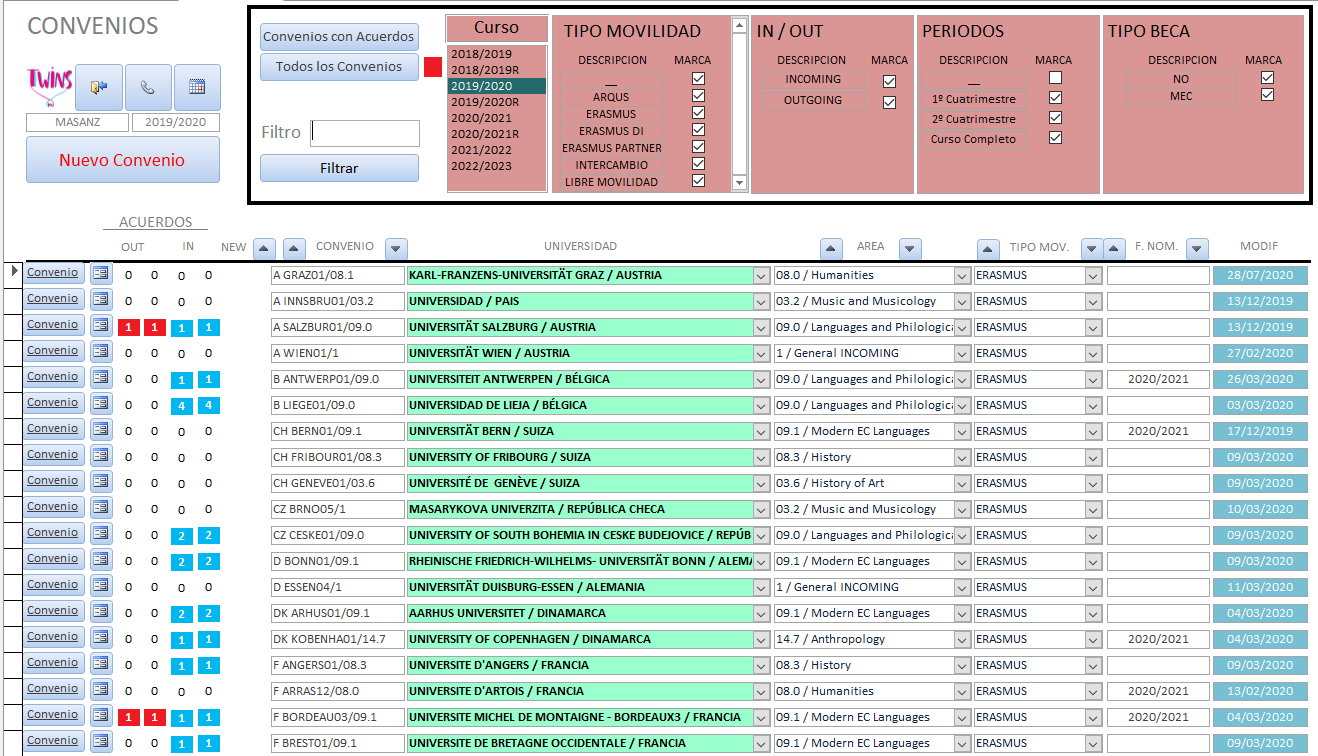
\includegraphics[width=\textwidth]{img/Capturas de TWINS/vistaConvenios.png}
	\caption{Vista de Convenios}
	\label{vistaConvenios}
\end{figure}

\begin{table}[h]
	\begin{center}
		\begin{tabular}{ | c | c | } 
			\hline
			\multicolumn{2}{|c|}{\textbf{Administración}} \\
			\hline
			Estudiantes \footnotemark & 2055 \\ 
			\hline
			Tutores & 58 \\
			\hline
			Convenios  & 607 \\ 
			\hline
			Expedientes & 5049 \\ 
			\hline
			\multicolumn{2}{|c|}{\textbf{Base de datos}} \\
			\hline
			Tablas & 108 \\
			\hline
			Relaciones & 60 \\
			\hline
			Macros & 55 \\
			\hline
			Formularios & 152 \\
			\hline
		\end{tabular}
		\caption{Estadísticas de TWINS}
		\label{estadisticasTWINS}
	\end{center}
\end{table}~
\footnotetext{Tanto \textit{incoming} como \textit{outcoming}}



\subsubsection{El modelo de datos}

El modelo relacional propuesto por Codd es el elegido para el diseño de esta base de datos. Las distintas tablas de la misma se conectan mediante relaciones que establecen restricciones para mantener la consistencia entre los datos.

Las tablas son una forma característica de almacenamiento de este modelo, en contraposición con otras disposiciones de la información usadas por otros sistemas y que, al fin y al cabo, se diseñan de otro modo porque se han de satisfacer unas necesidades distintas.

En este caso, podemos entender que la herramienta TWINS fue creada en Access y, por tanto, en un modelo de datos relacional dado el fácil acceso al usuario no experto en la materia, facilitando la operatividad con las bases de datos.

Es, sin duda, el modelo que más se utiliza aún hoy en día, el cual promete una determinada efectividad siempre y cuando el volumen de información a manejar no sea excesivamente elevado. En este caso, aunque la información que se requiere manipular en la oficina no es fácilmente manejable por personas, sí que aún podemos continuar utilizando este modelo para el desarrollo de la nueva herramienta twinX. Se entiende que no se tendrán más de unos 1000 estudiantes por curso académico (en una sola facultad) y que el número de convenios y tutores no será ni mucho menos parecido, considerando, eso sí, que la cantidad de \glspl{ExpedienteTWINS} será aproximadamente el doble que la de los estudiantes para los que se creen dichos registros.

Así pues, aparentemente, para las funcionalidades básicas y necesarias para trabajar en la oficina que twinX pretende implementar, el modelo relacional es suficiente.

No obstante, no olvidemos la intención de extender la funcionalidad del actual TWINS para que los propios estudiantes puedan dejar atrás el constante envío de documentos entre sus tutores académicos por correo electrónico, de modo que puedan dar el salto a una plataforma que implemente una interfaz que les permita prescindir de estos documentos, como el acuerdo de estudios, y trabajar con la información directamente (aunque se posibiliten las conversiones a certificados que puedan ser impresos). En este contexto, se ha de tener en cuenta la forma de tratar los datos que se quiere realizar. Si todas las asignaturas de la universidad de origen se tienen en memoria y tan sólo se tienen que registrar las de la universidad de destino, tan sólo tendríamos que guardar códigos, órdenes y los nuevos nombres para esas asignaturas. Sin embargo, si esto se complicara y tuviéramos que almacenar documentos, quizás, para esa parte de la aplicación, sería conveniente estudiar la posibilidad de implementar una base de datos cuyo modelo de datos esté enfocado a la búsqueda de estos y, no menos importante, optimizado para dicho propósito, algo que sería impensable en una base de datos relacional. Un ejemplo de estas bases de datos es \textbf{Elasticsearch}, que permite hacer búsquedas complejas en texto, a través de datos estructurados y desestructurados. Esta podría ser una buena opción a utilizar una vez se alcance una determinada complejidad en el sistema de almacenamiento, pero en nuestro caso, solo lo comentamos como posibles trabajos futuros.

\subsection{Funciones implementadas}

\subsubsection{Funcionalidades básicas}
Entre las funciones que hacen que TWINS cobre sentido, destacamos las siguientes:

\begin{itemize}
	\item \textbf{Almacenamiento de información administrativa:} estudiantes, tutores, convenios, expedientes, etc.
	\item \textbf{Asociación de estudiantes con otras entidades:} estudiantes con su tutor, el convenio respecto del cual realizan su movilidad, sus expedientes, etc.
	\item \textbf{\gls{AM}}: para poder organizar a los estudiantes \textit{incoming}
	\item \textbf{Envío masivo de correos electrónicos:} posibilita funciones como las \glspl{Nominacion} automáticas.
	\item \textbf{Generación de documentos automática:} disposición de los distintos datos en documentos que son entregables a estudiantes para mostrarles un sumario de su situación académica
	\item \textbf{Creación, edición y borrado de los datos dentro de la aplicación}
	\item \textbf{Anotación de futuras modificaciones a documentos ajenos a la oficina:} como son, por ejemplo, los convenios, que quedan registrados en la sede de la UGR y no pueden ser modificados hasta una fecha concreta, fuera del control de la oficina.
	\item \textbf{Recuperación de información de otros formularios externos a la aplicación:} para el registro de nuevos estudiantes (que es hasta ahora la mejor aproximación a la automatización de dicho proceso de la que se dispone) y, por ejemplo, para registrar datos de estudiantes afectados de alguna manera por la COVID-19.
\end{itemize}

\subsection{La interfaz de usuario}

Como hemos señalado en anteriores secciones, toda la aplicación yace sobre la herramienta de Microsoft\textregistered. Por ello, tanto los datos, como la presentación o vista y el control ejercido sobre los mismos no tiene separación alguna.

Al margen de esto y analizando las ventajas que el uso de Access\textregistered nos podría aportar, tenemos una manera de crear una interfaz de usuario de una manera más sencilla de lo normal. Tan sólo basta con arrastrar y redimensionar un botón con el ratón y una casilla para mostrar texto y con unas simples instrucciones tenemos una acción que, al pulsar el nuevo botón, en la casilla podría mostrarse, por ejemplo, cuántos registros almacena una determinada tabla (o varias de ellas) en la base de datos. Las consultas a la base de datos pueden almacenarse y reutilizarse según se quiera.

También pueden programarse como si de una consulta se tratara, acciones que impliquen la modificación, borrado o creación de registros en la base de datos. A estas piezas de código funcionales se les da el nombre de \textit{macros}.

Una vez mencionadas las posibilidades funcionales, abordemos el uso de las mismas que han hecho para construir TWINS.

Lo primero que nos encontramos tras abrir la aplicación, es una pantalla de login con los distintos usuarios que pueden acceder al sistema:

%imagen de login

Tras identificarnos, nos topamos, antes de llegar a la pantalla principal, con tres pantallas más:

\begin{itemize}
	\item La pantalla de avisos nos alerta de las acciones que tenemos que realizar con mayor urgencia, dado que han sido programadas para tenerlas listas para una fecha cercana y necesitan de la atención del usuario al que se notifica
	
	 %Imagen de avisos
	 
	\item La pantalla de notas, con los mensajes que se envían los distintos componentes de la oficina entre ellos, funciona como un paso de notas adhesivas que se dejan en los distintos puestos de trabajo. Sólo el administrador puede ver todas las notas que todos los usuarios se envían, pero son privadas a emisor y receptor del mensaje. Eso sí, hablamos de la vista, porque ya que todo el mundo necesita el archivo de base de datos para interaccionar con ella, todo poseedor puede abrir la tabla de mensajes y ver todo su contenido.
	
	%Imagen de mensajes
	
	%Otra pantalla que falta
	
	%Su imagen
	
\end{itemize}

Finalmente, llegamos a la pantalla principal, de donde parten todos los menús (incluso los que acabamos de ver, que disparan su vista al ser satisfactorio el proceso de identificación en el sistema).

%Imagen de pantalla principal

En ella, no vemos ninguna información como la que acabamos de ver ahora (ni indicador de notificaciones, mensajes, alertas; nada). Lo que sí podemos apreciar es una selección en la parte de arriba de la interfaz con la que se filtrará el contenido que aparezca tras acceder a cualquier elemento del menú. Esto es, se filtrarán las consultas que se hagan, pues al fin y al cabo es en lo que consiste la recuperación de parte de la información almacenada en la base de datos.

\section{Estudio de necesidades}
